% options:
% thesis=B bachelor's thesis
% thesis=M master's thesis
% czech thesis in Czech language
% english thesis in English language

\documentclass[thesis=M,english]{FITthesis}[2011/07/15]

% \usepackage[utf8]{inputenc} % LaTeX source encoded as UTF-8
% \usepackage[latin2]{inputenc} % LaTeX source encoded as ISO-8859-2
% \usepackage[cp1250]{inputenc} % LaTeX source encoded as Windows-1250

\usepackage{graphicx} %graphics files inclusion
\usepackage{algorithmic} %subfigures
% \usepackage{amsmath} %advanced maths
% \usepackage{amssymb} %additional math symbols

% % list of acronyms
% \usepackage[acronym,nonumberlist,toc,numberedsection=autolabel]{glossaries}
% \iflanguage{czech}{\renewcommand*{\acronymname}{Seznam pou{\v z}it{\' y}ch zkratek}}{}
% \makeglossaries

\usepackage{listings}
\usepackage{color}

\definecolor{dkgreen}{rgb}{0,0.6,0}
\definecolor{gray}{rgb}{0.5,0.5,0.5}
\definecolor{mauve}{rgb}{0.58,0,0.82}
\definecolor{lightgray}{rgb}{0.93,0.93,0.93}

\lstset{frame=none,
  language=C,
  aboveskip=3mm,
  belowskip=3mm,
  showstringspaces=false,
  columns=flexible,
  basicstyle={\small\ttfamily},
  numbers=left,
  numberstyle=\tiny\color{gray},
  keywordstyle=\color{blue},
  commentstyle=\color{dkgreen},
  stringstyle=\color{mauve},
	backgroundcolor=\color{lightgray},
  breaklines=true,
  breakatwhitespace=true
  tabsize=3
}

% % % % % % % % % % % % % % % % % % % % % % % % % % % % % % 
% EDIT THIS
% % % % % % % % % % % % % % % % % % % % % % % % % % % % % % 

\department{Department of \ldots (SPECIFY)}
\title{Thesis title (SPECIFY)}
\author{Pavel Kachalouski} %author's name without academic degrees
\authorWithDegrees{Pavel Kachalouski \& degrees} %author's name with academic degrees
\supervisor{Your Supervisor's Name (SPECIFY)}
\acknowledgements{THANKS}
\abstractEN{Summarize the contents and contribution of your work in a few sentences in English language.}
\abstractCS{V n{\v e}kolika v{\v e}t{\' a}ch shr{\v n}te obsah a p{\v r}{\' i}nos t{\' e}to pr{\' a}ce v {\v c}esk{\' e}m jazyce.}
\placeForDeclarationOfAuthenticity{Olomouc}
\keywordsCS{Replace with comma-separated list of keywords in Czech.}
\keywordsEN{Replace with comma-separated list of keywords in English.}

\parskip 2mm

\begin{document}

% \newacronym{CVUT}{{\v C}VUT}{{\v C}esk{\' e} vysok{\' e} u{\v c}en{\' i} technick{\' e} v Praze}
% \newacronym{FIT}{FIT}{Fakulta informa{\v c}n{\' i}ch technologi{\' i}}

% \setsecnumdepth{part}
\chapter{Introduction}
\section{Motivation}
First major malicious internet-based attack was introduced in 1988 when one of the first Internet worms was released. Referred to as "The Morris Worm", it was written by Robert Tappan Morris and caused major interruptions across large parts of the Internet. Since 1988 Internet has greatly evolved and as a result increased number of internet-based attacks and network security became a really important issue. As an attempt to overcome this problem Intrusion Detection systems were developed. Such systems allow to monitor and possibly prevent attempts to intrude into or compromise the network resources.

In short it works as follows: you have a computer system. Your computer system is attached to the network and may be even to the Internet. You are willing to allow access from the network, by authorized people, but you are not however willing to allow unauthorized access to the system by anyone else. Typically, a firewall or authentication system is used to prevent unauthorised access. However, sometimes authentication systems and firewalling can be broken. Intrusion Detection is a set of mechanisms that are helps to detect unauthorised access to the system. Also Intrusion Detection systems may take some steps to deny access for intruders. Such systems are placed between firewall and system being secured and provide an extra layer of protection to that system.
\begin{figure}[h]
\centering
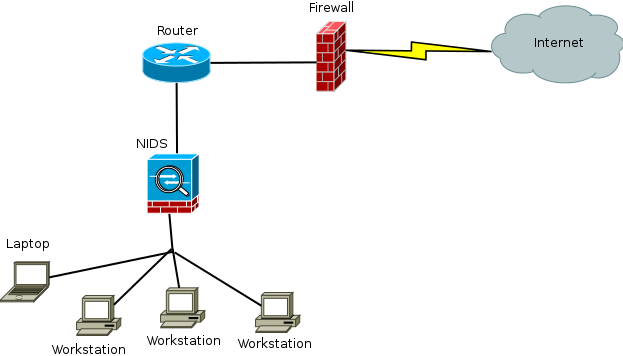
\includegraphics[scale=0.5]{images/Typical_NIDS.png}
\caption{Typical NIDS scenario.}
\label{fig:typical_nids}
\end{figure}
Intrusion detection systems fall into two categories:
\begin{itemize}
\item Network based system. 
Such types of systems are placed in the network near the system that should be monitored. They monitor network traffic and examine whether it is withing acceptable boundaries.
\item Host based systems. 
Such types of detection systems are run on the system being monitored and determine if activity on the system is acceptable.
\end{itemize}
There are also more recent type of intrusion detection system which reside in the kernel of operation system and monitor on low-level system activity.

Most modern network intrusion detection and prevention systems use a set of rules that are compared to incoming and outcoming packets. Usually, a rule consists of a filter based on packet header information, a data that should be contained in the packet payload and an associated action that is taken in case filter and payload matching conditions are met.
Matching payload signatures is a resource-intensive process, accounting for about 75\% of the total CPU processing time of modern Network Intrusion Detection systems. The reason why is it so intensive is in the fact that most of the time, every byte of every network packet should be processed as a part of data searching algorithm that searches for matches along a large set of rules that apply for particular packet. As an example, most widely used open-source NIDS Snort has rule set with about 10000 strings. Searching every packet for all of this strings needs a lot of resources. 
\begin{figure}[h]
\centering
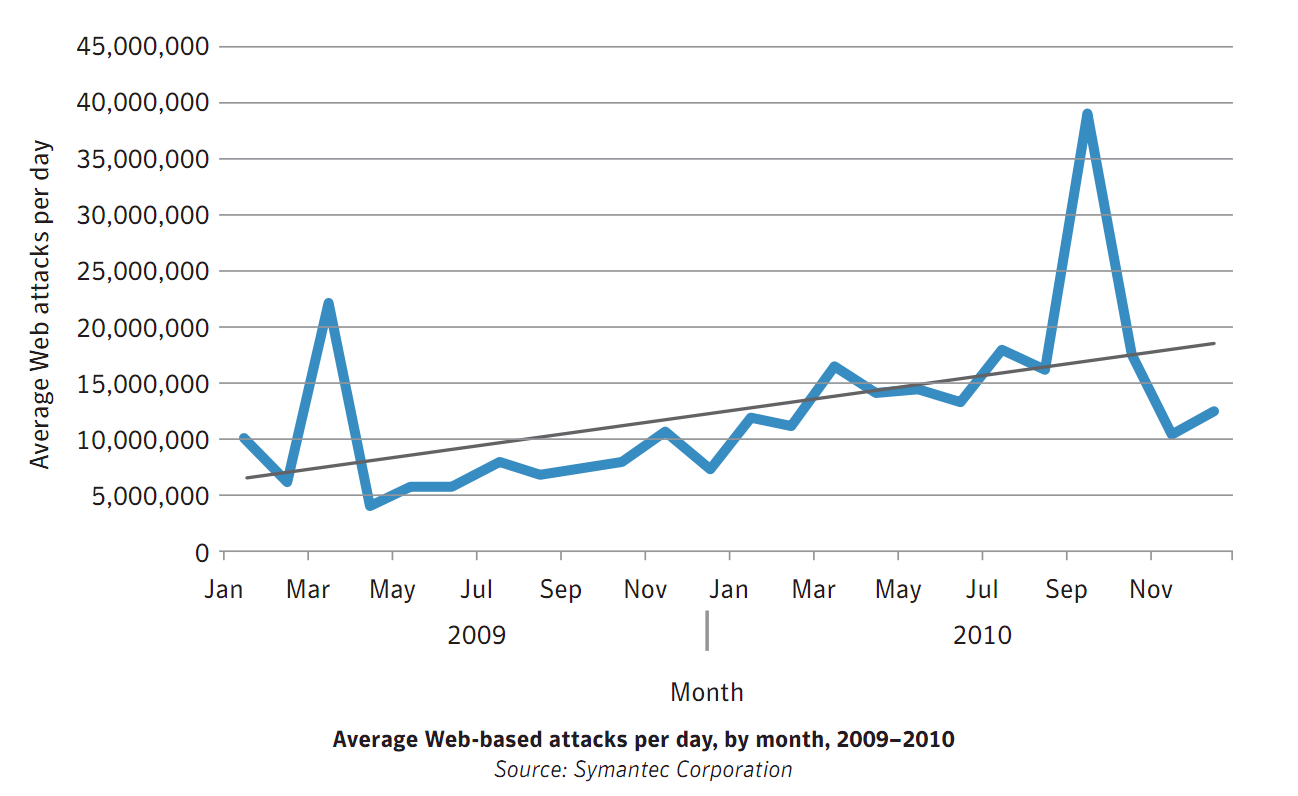
\includegraphics[scale=0.3]{images/web-attacks.png}
\caption{Average Web-based attacks per day, by month, 2009-2010. Source: Symantec Corporation.}
\label{fig:symantec_report}
\end{figure}
With increasing number of internet-based attacks rules datasets grow every year creating additional load on NIDS systems. Figure \ref{fig:symantec_report} shows a general trend of the number of web-based attacks on web servers taken from Symantec Corporation report.

The other source of high load on NIDS is constant grow of networks speeds. In the past 6 years, computer networks were characterized by a steady increase in the transfer rate, complexity and number of networked users. In 2009 the Internet traffic growth all over the world amounted to 40-50 \%, and according to Cisco company forecast [TODO:add number] global IP traffic will increase in the next 5 years, reaching by 2015 about 1 zettabyte of data transferred during one year.

Problem with high load on NIDS can be solved by using specialized network processing devices such as FPGA, ASIC, Network Processing Unit (NPU), or the TCP Offoading Engine (TOE). Nonetheless, the solutions may not be cost effective and easy to manage because they require special hardware and configurations.

\subsection*{Problem definition}
A quick packet processing in a NIDS over huge amount of data obtained from the network \textbf{is a must}. Perfomance of network data processing algorithms should be fast and should not interfere with the overall network perfomance (or interfere as little as possible).
The current factors related to the networks and traffic analysis systems listed below:
\begin{enumerate}
\item The number of network nodes and users are increasing. 
\item Network speed (bit rate) is gradually increasing.
\item The amount of network traffic is increasing heavily.
\item Analysis algorithms are getting more complex.
\item Databases of known threats grow resulting in high number of rules for matching.
\end{enumerate}

This thesis approach is to use heterogeneus computing, and more specifically use \textbf{graphic processing units} to perform network data analysis.

Heterogeneous computing is a way of computing some tasks using systems made up by different types of computational units. Computational unit types could be: a general-purpose processors (GPP), also known as central processor units (CPUs), which are usually the main processor of the most of the computing systems, and special-purpose processors (SPP). SPP are, for example, digital signal processors (DSP) or graphics processor units (GPU).

Graphics Processing Unit or GPU is essentially a dedicated hardware device that is responsible for translating data into a 2D image formed by pixels. GPU evolution is connected to the growing popularity and complexity of rendering programs like CAD (Computer Aided Design) programs and to 3D video games. These software required high computing capabilities which have to be satisfied by the GPUs. As a result engineers developed a highly parallel processor structure, which is able to execute many execution threads concurrently, and a high speed memory.

The interest to use GPUs to perform calculation tasks that are not suitable for GPUs began to grow in 2005. Developers and investigators were trying to use parallelism and memory bandwidth to enhance complex algorithms perfomance. GPUs are used for computations in molecular dynamics, quantum chemistry, bioinformatics, computational fluid dynamics, weather and climate forecasting and more other fields.

GPGPU (general-purpose computing on graphics processing units) at the beginning used GPUs as they were computing graphics tasks. Input data were encoded into image, then by using graphics libraries some operations were perfomed with an image and result data were decoded from image to its original form. Later companies realised that GPGPU could be an advantage for their business and invested in developing tools to make easier to use their products. NVIDIA developed CUDA (an acronym for Compute Unified Device Architecture) version 1.0 library in 2006, which enabled to run CUDA code written in special manner on some of their GPUs, while AMD developed ATI Stream technology that uses OpenCL language to write code executed on GPUs.

CUDA is the computing engine in Nvidia GPUs that is accessible to software developers through variants of industry standard programming languages. Programmers use 'C for CUDA' (C with Nvidia extensions and certain restrictions), compiled through a PathScale Open64 C compiler to code algorithms for execution on the GPU.
The main objective of this thesis is to develop open-source NIDS application which will inspect network traffic using classic CPU mode and heterogeneous CPU+GPU mode and compare perfomance of the two modes. 

In additional, the software should fulfill the following requirements:
\begin{itemize}
\item Open source. The application should be developed under the terms of open source software.
\item Application should be developed in C/C++ and C for CUDA languages.
\item Easy to use. Application should be easy to use for the users. NIDS rules should have easy format.
\item Application will analyze only TCP/IP traffic due to simplifications on the packet decomposition level.
\item Logging and offline analysis. Application should be able to store traffic for the future analysis in offline mode.
\end{itemize}

\section{Project overview}

The general application workflow is shown in the figure \ref{fig:app_workflow}.
\begin{figure}[h]
\centering
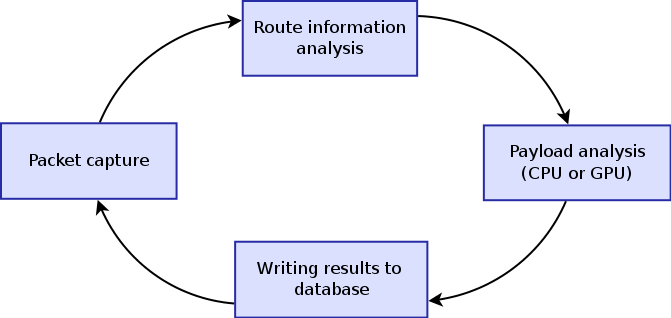
\includegraphics[scale=0.4]{images/workflow.png}
\caption{Application workflow.}
\label{fig:app_workflow}
\end{figure}

The main stages of the workflow:
\begin{itemize}
\item \textbf{Packet capture}. Application captures traffic on one of the network interfaces for later analysis. Raw packet should be obtained from network for full analysis of route information on the next stage.
\item \textbf{Route information analysis}. Every packet is analyzed by means of type of the protocols used on network and transport layers and also destination and source IP address. If packet route information matches to any rule from the dataset it transported to the next stage of the workflow.
\item \textbf{Payload analysis}. Application looks for a string or regex in the packet payload.
\item \textbf{Writing result to a database}. On this stage all matched packets from the previous stage are written to a database with a message obtained from rule with which packet was matched.
\end{itemize}

\chapter{Background}
\section{Traffic analyzing: sniffers.}
Packet sniffer is a program or library which allows to intercept data packets transmitted over a certain network to which the system is connected throught a network card. Most popular known sniffing software is tcpdump[], Wireshark and OmniPeek. These programs are used for obtaining raw network packets and performing analyzing over obtained packets in order to represent them in a some visual form or dump to a file. There are also pure sniffing libraries, such as Libpcap (for UNIX like OS) and Winpcap (for Windows OS).

\subsection{How they work.}
The vast majority of network cards, support what is known as promiscuous mode or monitor mode. Normal operation of network cards when obtaining packets from the network (default configuration), compare the destination layer 2 (link layer) address to the one in use by the network card. If packet destination address and network card address in use match, or if the packet destination address is a broadcast address 1, packets are passed to the operating system, otherwise packets are dropped.

If promiscuous mode or monitor mode is enabled, network card passes all packets captured from the network to the operating system, even if they are not addressed to the system. Operating system later manages, using the packet filter engine, how to distribute packets to the applications. In the Unix-like systems, root privileges are required to enable promiscuous and monitor operation mode. Sniffer techniques rely on this functionality to do its job.

It is important to remark that capturing packets from a network is highly dependent of the type of the network used and of the topology and configuration of the network. Clear examples of this fact can be found in LAN (Local Area Network) networks based on the IEEE 802.XX (physical and link layer protocols) protocol macro-family, for instance in the IEEE 802.3 protocol based networks, also known as Ethernet networks, and in the IEEE 802.11 based networks, so-called Wifi or Wireless networks. In the following subsections some details over sniffing on both network types are exposed.

\subsection{Packet capture in IEEE 802.3 networks.}
In a typical IEEE 802.3 LAN network, a star topology is used, so all the nodes in the network are connected (through their own cable) to either a hub or a switch.
\begin{figure}[h]
\centering
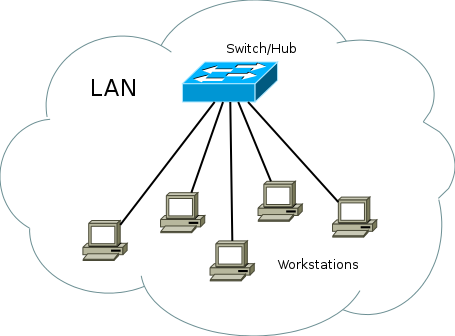
\includegraphics[scale=0.45]{images/IEEE802_3_LAN.png}
\caption{IEEE 802.3 networks usually use star topology.}
\label{fig:ieee802.3star_topology}
\end{figure}

Hubs are basically repeaters: packets coming from a certain port are retransmitted over the rest of the ports.
Switches instead, only send packets to the port where the destination host is connected, by previously identifying all the hosts connected to each port. Switched networks have better performance than not switched networks. Switches may perform other actions over traffic, such as filtering based on different protocol fields (link, network, transport and application protocol fields, depending on the switch), but this is beyond the scope of this thesis.
That means that if a switched network is used, only packets flowing to or from the particular host running the sniffer or broadcast packets will be captured. Several techniques have been used to overcome this problem:
\begin{itemize}
\item Using a hub: an obvious but bad solution is to use hubs instead of switches. It is not a valid solution as its performance is very reduced compared to switched networks and their production is practically discontinued.
\item Placing the sniffer in the gateway links as a bridge/router: this technique is widely used and has the advantage of being able to sniff packets from a lot of sub-networks by only placing one network tap. The disadvantage is that only traffic going through that link is captured, so internal traffic (between nodes in the same subnetwork or between different sub-networks) is not captured, which in some cases, like data centers for instance, is very relevant. 
\begin{figure}[h]
\centering
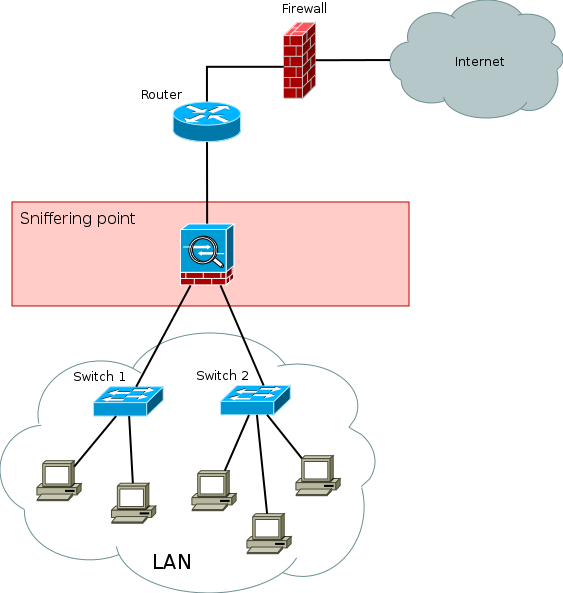
\includegraphics[scale=0.6]{images/gateway_sniffering.png}
\caption{Sniffering traffic in the gateway links.}
\label{fig:gateway_sniffering}
\end{figure}
In those cases the only solution is to use distributed sniffers, port mirroring or a combination of both of them. Figure \ref{fig:gateway_sniffering} illustrates this technique with an example.
\item Switch port mirroring: some switches have what is called port mirroring or monitoring port 2. If port mirroring is enabled, a copy of all the packets flowing in the switched are transmitted to the mirroring port selected. On networks formed by several switches, obtaining packets in a single host is more complex, and may require to use advanced switch capabilities like Cisco’s RSPAN or combine them with a distributed sniffer.
\begin{figure}[h]
\centering
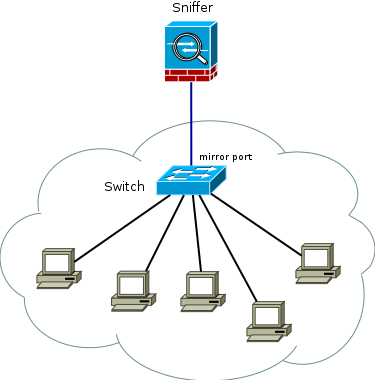
\includegraphics[scale=0.6]{images/mirror_sniffering.png}
\caption{Sniffering traffic using switch port mirroring.}
\label{fig:mirror_sniffering}
\end{figure}
\item Distributed sniffer: distributed sniffers use a software based architecture to collect traffic in several network taps (hosts), and combine them to obtain them in a unique host. The main advantages of this type of systems are their scalability and flexibility. The drawbacks of this kind of systems are that distributed network sniffers have less performance than port mirroring due to overhead introduced by software architecture and the increase of network traffic. The figure \ref{fig:distributed_sniffering} shows graphically the structure of a distributed sniffer platform.
\begin{figure}[h]
\centering
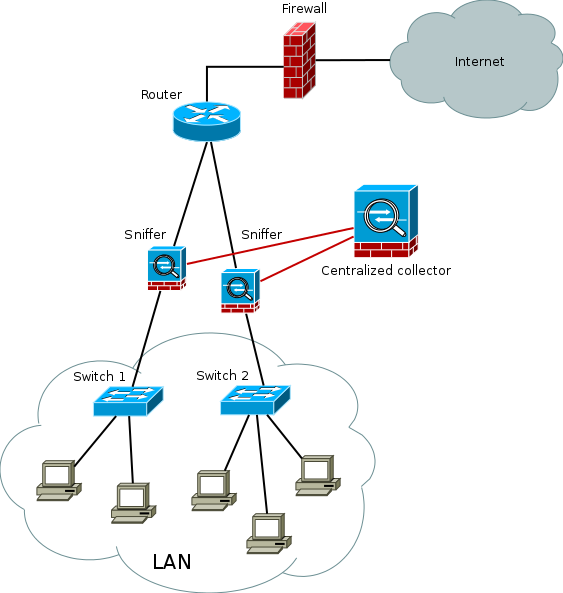
\includegraphics[scale=0.6]{images/distributed_sniffering.png}
\caption{Distributed sniffer.}
\label{fig:distributed_sniffering}
\end{figure}
\end{itemize}
\subsection{Packet capture in IEEE 802.11 networks.}
IEEE 802.11 based networks share access medium, so it may be easier than IEEE 802.3 switched networks to capture packets, as having a network card being able to be set to promiscuous mode (actually monitor mode) is all the hardware required.
Nevertheless, some considerations have to be kept in mind. When placing a sniffer in a wireless network, some packets or even all the packets sent by a certain host may be lost, due to environment conditions (shadowing) and the physical position of the sniffer host and the other hosts in the network (attenuation due to propagation). IEEE 802.11 networks made up by several access points may increase capturing problems, due to the larger coverage area (and therefore the higher reception antenna gain needed when using a unique sniffer host).
Some approaches to solve these problems are:
\begin{itemize}
\item Capture packets in the wired network section: sometimes is preferable to sniff packets in the wired section rather than capturing them in the wireless subnetwork. This is conceptually similar to place a sniffer in the gateway link above mentioned, so the main disadvantage is that internal wireless traffic is not captured. This approach has also the drawback that link layer protocol (level 2) information is lost.
\item Distributed sniffer: usage of distributed systems. Pros and cons are similar than above mentioned.
\end{itemize}

\subsection{Libpcap.}
Libpcap is the capture library for Unix systems. Windows systems use a port of Libcap called Winpcap. This library offers the programmer an API to use BSD Packet Filter kernel facilities or any other Packet Filter kernel architecture that is based on Berkeley Packet Filter, to create user-level network capturing programs. Libpcap was released by the tcpdump developers in the Network Research Group at Lawrence Berkeley Laboratory. Libpcap offers the following capabilities: packet capturing from a network card, packet capturing from a file and capturing packets to save them into a file. Libpcap was extracted from the tcpdump program and made into a library. Development of Libpcap is in charge of tcpdump group [TODO: add number].

\subsection{Network traffic analysis techniques.}
In this section a brief introduction of main network traffic analysis techniques currently in use is exposed, focusing on the analysis procedures but also outlining some of the
analysis purposes which take advantage of them. But first, some considerations over the network traffic analysis inputs (network data) should be sketched out. The main input source of any network traffic analysis is the collection of packets captured from the network, commonly called the dataset or the analysis dataset. From that dataset which may contain all protocol header information as well as application an user information, a process of extracting (mining) the useful pieces of data for every particular analysis has to be carried out.
Datasets may also be broken up in smaller parts, resulting in data subsets, to later be analysed separately. The reasons of splitting dataset are usually performance issues with non-linear computing cost analysis algorithms, as working with large datasets may increase computing time exponentially, or to achieve a higher time resolution due to the reduced time interval of the datasubset. In these cases analysis are said to be performed over windowed datasets or simply called windowed analysis. Depending on the criteria followed to split the dataset into data subsets, two different types of windowed datasubsets can be obtained:
\begin{itemize}
\item Packet windowed datasubsets. Dataset is splitted in portions of equal number of packets each.
\item Time windowed datasubsets. Dataset is splitted in time intervals. The size of the subsets is unknown, and depends on the amount of traffic collected per second.
\end{itemize}

The usage and type of dataset windowing may affect to the results of the different analysis performed over it, and hence windowing parameters have to be taken into account when analysis results have to be evaluated and interpreted.

\subsection{Network traffic data inspection techniques.}
Network data inspection techniques obtain information of network data by inspecting network header fields of each packet, compute them and produce outputs or results.

\textbf{Packet decoding (packet analyzing)}
The simplest network data inspection possible is packet decoding, also called packet analysis, in which all header’s field are decoded and presented in a human readable way. Network analyzers like tcpdump, Wireshark or OmniPeek are some examples of packet decoding applications.
Packet decoding is used for the vast majority of purposes, being the most reliable security (intrusion detection, bandwidth abuse...) and network management and failure detection.
This kind of techniques are specially of interest in network security forensics analysis. Specific packet data extraction and analysis The extraction of pieces of data from the packets contained in the dataset instead of decoding all packet headers information, and processing them is a strategy used when particular aspects of traffic need to studied.
Different processing tasks can be performed over data collected:
\begin{itemize}
\item Graphical representation of raw data.
\item Statistical information and pattern extraction
\item Rule based (signature based) analysis, anomaly detection and policies.
\item Flow based analysis.
\end{itemize}
Graphical representation of raw data is of interest in many areas, principally in network monitoring, network management and security. Representations are usually in the form of 2D and 3D scatter plots, time based graphs, histograms, pie charts or diagrams. Network monitoring applications make an extensible usage of graphs like node state monitor graphs, throughputs and link performance graphs, source and destination hosts (IPs) histograms and scatter plots, service usage (TCP and UDP ports) histograms and scatter plots or routing diagrams. Some examples are shown in the figures below.

Statistical information and pattern extraction is a big field in network analysis. First and second order statistical moments, averages, time distributions and probability distributions functions are some of the basic statistical analysis that can be performed over network data. 
Obtaining interesting statistics over network traffic is widely used primarily in monitoring platforms. Average number of connections to a certain hosts, average inbound and outbound throughputs, transport and application layer protocol distribution, time distribution of connections to servers, time distribution of average network throughput are some examples. These statistics can also be applied for other purposes rather tan monitoring and network management, like security or marketing purposes (specially application level statics).

On the other hand, statistical pattern recognition or statistical pattern extraction is an extensive area related to network traffic analysis. They are applicable to security and
marketing fields. Due to the extension of this field and complexity, further information is given in the 2.2.2.2 section. Rule based (signature based) analysis and policies are all the analysis that inspect traffic searching packets that match a certain rule or signature. Rules or signatures are defined as values of certain headers fields or a combination of several values of certain headers fields. Rules may also define adequate field value intervals or thresholds. Rule based analysis is also frequently called signature pattern matching. There is quite a confusing usage of the term pattern over the network analysis literature, and particularly in network intrusion detection analysis literature: while some authors use the word pattern to designate statistical patterns (statistical user behaviour patterns, statistical usage patterns in general) like W.S. Chen in or Yung Wang in, some others like Richard Bejtlich in several books like use them to refer as rule based analysis. In this thesis be are going to refer to patterns as statistical patterns only. Rule based analysis techniques are used above all for security purposes and specially in signature based intrusion detection systems (NIDS), like Snort. Threshold rules are commonly used in security (for instance to detect DoS attacks and other resource abuse attacks) and also for network management purposes like for example in network link load monitoring.

In this sense, rules could be considered as policies, as certainly define the type and amount of traffic permitted and not permitted in the network. Flow based analysis techniques are focused in the treatment of network traffic as flows, as most information exchanged in a computer network is session or connection oriented and not packet oriented, so analysis can take advantage of it. A clear example of a typical network flow is a TCP connection, where data exchanged is ruled by the TCP state machine.
Their main applications are in the monitoring and security field. Regarding security, most NIDS like Snort, use flow based analysis techniques to detect possible threats, based on anomalies and well known attacks. Monitoring platforms on the other hand, inspect network traffic in search of flows, to generally list them or represent them in a diagram.

\textbf{Advanced statistical and signal processing techniques applied to the network traffic analysis.}
Since early 1990’s, researchers all over the world have devoted some of their efforts in the research of advanced statistical analysis techniques and also applying signal processing techniques to the network traffic analysis. The efforts have been centered in the network intrusion detection and prevention field, due to the fact that signature based NIDS (and NIPS) have important limitations detecting new security threats, as new rules for detection appear as new attacks and security threats are discovered. In addition,
signature based NIDS have the obvious drawback that rulesets have to be frequently updated. Platforms or applications that use statistical techniques for the network intrusion de-
tection are known as Statistical Network Intrusion Detection Systems or alternately Behaviour based Network Intrusion Detection Systems. This kind of NIDS rely on advanced statistical techniques, heuristic pattern extraction and signal processing to detect anomalies and classify network traffic.

Y. Wang exposes in his book a general and up to date state-of-the-art of most reliable statistical techniques in the field of statistical network intrusion detection. There
is also an extensive set of publications from researchers over new statistical and signal processing techniques applied to network intrusion detection. Some of the techniques
are briefly introduced here.

\textbf{Linear and Nonlinear modeling methods.}
Significance tests, like $\chi^2$ (chi-square) test and t-test have been proposed for a simple network intrusion detection, examining frequency difference between two categorical variables and differences between two continuous variables respectively. Linear methods like logistic models, regression models, principal component analysis or clustered based analysis are some of the main methods suitable to use complex statistical modeling techniques to examine user behaviour based on network traffic data. 
Non linear methods are fundamentally based in AI (artificial intelligence) algorithms like Artificial neural networks, Fuzzy logic algorithms and K-nearest neighbour algorithms have also been found effective for aiding network intrusion detection decisions.

\textbf{Bayesian and probability approaches.}
Bayesian and probability approaches assume that parameters that are being studied are random rather than fixed parameters. Before looking at the current data, old information can be used to construct a prior distribution model for these parameters and therefore classify new data based on how likely various values of the unknown parameters are, and then make use of the current data to revise this starting assessment so that parameters can be considered random, not fixed. This attribute allows an intrusion detection systems to make a more precise decision based on the probability approach. Latent class model based analysis like proposed in Wang, Kim, Mbateng and Ho or Bayes role based analysis like proposed by Barbard, Wu and Jajodia are some examples of Bayesian and probability approaches.

\section{Intrusion detection.}
Intrusion detection is a process of detection undesired traffic on a network or device. An Intrusion Detection System is a combination of a physical device with a software which monitors network traffic in order to detect undesired activity and traffic that violates security policies. Different IDS tools are able also to store event information into log for later review or combine events with other information to make decisions about policies and losses. More functionalities provide IPS that can prevent or stop undesired traffic.

\textbf{Network-based Intrusion Detection (NID)}

A Network Intrusion Detection System (NIDS) is a type of IDS that monitors network traffic and analyzes packets deep on all levels of OSI model. Based on result of analyzis it makes decisions about the traffic type and suspicious activity. However, historically NIDS has been unable to operate in the following environment:
\begin{itemize}
\item Switched networks.
\item Encrypted networks.
\end{itemize}

\textbf{Host-based Intrusion Detection (HID)}

Host-based intrusion detection systems monitor and detect system and user activities on a given host. More complicated tools also offer policy management, data forensics statistical analysis and some access control. The difference between network-based intrusion detection and host-based intrusion detection is that NID deals with a traffic transmitted from one host to another while HID controls what is happening on the hosts themselfs.

Host-based intrusion detection is better fits to fight with internal threats, because it monitor and control specific user actions and file access. A lot of computer threats comes from the inside of organization, for example disgruntled employees or corporate spies.

\subsection*{Detection types}

\textbf{Signature-Based Detection}

Intrusion Detection may use signature-based detection to analyze traffic. Using such type of detection means that system is relying on known traffic data to analyze running traffic. An attacker can modify a little an attack to make it undetectable for such type of IDS. But regular expression-based rules give more power against such slightly changed attacks in the same time remaining very accurate.

\subsection*{Anomaly-Based Detection}
An IDS that looks at network traffic and detects data that is incorrect, not valid, or generally abnormal. This method is useful for detecting undesired traffic that is not specifically known. For instance, an anomaly-based IDS will detect that an Internet protocol (IP) packet is malformed. It does not detect that it is malformed in a specific way, but indicates that it is anomalous.

\subsection*{Stateful Protocol Inspection}
This type of detection is similar to anomaly-based detection, but it additionally inspects traffic on the transport layer and vendor-specific application layer, while anomaly-based detection is not doing it.

\section{Intrusion Detection Systems: A Brief History.}
The goal of intrusion detection is to monitor network assets to detect anomalous behavior and misuse. This concept has been around for nearly twenty years but only recently has it seen a dramatic rise in popularity and incorporation into the overall information security infrastructure. Beginning in 1980, with James Anderson's paper, Computer Security Threat Monitoring and Surveillance, the notion of intrusion detection was born. Since then, several pivotal events in IDS technology have advanced intrusion detection to its current state.

James Anderson's seminal paper, written for a government organization, introduced the notion that audit trails contained vital information that could be valuable in tracking misuse and understanding user behavior. With the release of this paper, the concept of "detecting" misuse and specific user events emerged. His insight into audit data and its importance led to tremendous improvements in the auditing subsystems of virtually every operating system. Anderson's conjecture also provided the foundation for future intrusion detection system design and development. His work was the start of host-based intrusion detection and IDS in general.

In 1983, SRI International, and specifically Dr. Dorothy Denning, began working on a government project that launched a new effort into intrusion detection development. Their goal was to analyze audit trails from government mainframe computers and create profiles of users based upon their activities. One year later, Dr. Denning helped to develop the first model for intrusion detection, the Intrusion Detection Expert System (IDES), which provided the foundation for the IDS technology development that was soon to follow.

In 1984, SRI also developed a means of tracking and analyzing audit data containing authentication information of users on ARPANET, the original Internet. Soon after, SRI completed a Navy SPAWAR contract with the realization of the first functional intrusion detection system, IDES. Using her research and development work at SRI, Dr. Denning published the decisive work, An Intrusion Detection Model, which revealed the necessary information for commercial intrusion detection system development. Her paper is the basis for most of the work in IDS that followed.

Meanwhile, there were other significant advances occurring at University of California Davis' Lawrence Livermore Laboratories. In 1988, the Haystack project at Lawrence Livermore Labs released another version of intrusion detection for the US Air Force. This project produced an IDS that analyzed audit data by comparing it with defined patterns. In a telephone interview with the author, Crosby Marks, a former Haystack Project team member and Haystack Labs employee said that, "searching through this large amount of data for one specific misuse was equivalent to looking for a needle in a haystack."

The subsequent iteration of this tool was called the Distributed Intrusion Detection System (DIDS). DIDS augmented the existing solution by tracking client machines as well as the servers it originally monitored. Finally in 1989, the developers from the Haystack project formed the commercial company, Haystack Labs, and released the last generation of the technology, Stalker. Crosby Marks says that "Stalker was a host-based, pattern matching system that included robust search capabilities to manually and automatically query the audit data." The Haystack advances, coupled with the work of SRI and Denning, greatly advanced the development of host-based intrusion detection technologies.

To kick off the '90s, UC Davis's Todd Heberlein introduced the idea of network intrusion detection. In 1990, Heberlein was the primary author and developer of Network Security Monitor (NSM), the first network intrusion detection system ( see Heberlein, L. et al. "A Network Security Monitor." Proceedings of the IEEE Computer Society Symposium, Research in Security and Privacy, May 1990, pp. 296-303.) NSM was deployed at major government installations where network traffic analysis provided massive amounts of information. This new awareness generated more interest in the field of intrusion detection and investments in that market increased significantly. Heberlein's contributions also extended to the DIDS project where, along with the Haystack team, he introduced the first idea of hybrid intrusion detection. The work of the Haystack project and the introduction of the Network Security Monitor revolutionized the IDS field and brought it into the commercial world.

Commercial development of intrusion detection technologies began in the early 1990s. Haystack Labs was the first commercial vendor of IDS tools, with its Stalker line of host-based products. SAIC was also developing a form of host-based intrusion detection, called Computer Misuse Detection System (CMDS). Simultaneously, the Air Force's Cryptologic Support Center developed the Automated Security Measurement System (ASIM) to monitor network traffic on the US Air Force's network. ASIM made considerable progress in overcoming scalability and portability issues that previously plagued NID products. Additionally, ASIM was the first solution to incorporate both a hardware and software solution to network intrusion detection. ASIM is still currently in use and managed by the Air Force's Computer Emergency Response Team (AFCERT) at locations all over the world. As often happened, the development group on the ASIM project formed a commercial company in 1994, the Wheel Group. Their product, NetRanger, was the first commercially viable network intrusion detection device. Nonetheless, commercial intrusion detection systems developed slowly during these years and only truly blossomed towards the latter half of the decade.
The intrusion detection market began to gain in popularity and truly generate revenues around 1997. In that year, the security market leader, ISS, developed a network intrusion detection system called RealSecure. A year later, Cisco recognized the importance of network intrusion detection and purchased the Wheel Group, attaining a security solution they could provide to their customers. Similarly, the first visible host-based intrusion detection company, Centrax Corporation, emerged as a result of a merger of the development staff from Haystack Labs and the departure of the CMDS team from SAIC. From there, the commercial IDS world expanded its market-base and a roller coaster ride of start-up companies, mergers, and acquisitions ensued. (The next section, Players, discusses these developments.)

Currently, market statistics show that IDS is amidst the top selling security vendor technologies and should continue to rise. Furthermore, government initiatives, such as the Federal Intrusion Detection Network, (FIDNet) created under Presidential Decision Directive 63, are also adding impetus to the evolution of IDS. Advancements in IDS will ultimately push security technology into a whole new arena of automated security intelligence.

\section{GPUs}
GPU is a graphical processor unit sometimes also called visual processing unit or VPU, is a specialized type of processor that is responsible to render 3D graphics and offload this procedure from the micriprocessor or CPU. GPU history starts in 1970s, when ANTIC and CTIA chips were provided for hardware control of mixed graphics and text mode on Atari 8-bit computers. The ANTIC chip was a special purpose processor, that was responsible for mapping graphics and text data to the video output.

Later, in 1984 the IBM Professional Graphics Controller appeared as one of the first 2D/3D graphics accelerators available for the IBM PC architecture compatible systems. IBM’s chip did not succeed, due to the lack of compatibility with already existing programs and due to its high price. Commondore Amiga was the first mass-market computer which included a dedicated graphics processor launched in 1985. Amiga's graphic processor was the first full graphics accelerator that offloaded practically all video operations from th CPU.

The first graphics system that implemented 2D primirives in hardware was the IBM's 8514 PC video card. In 1991, S3 manufacturer introduced the S3 86C911 to the market, which claimed to be the first single-chip graphics card to implement 2D acceleration functions in hardware. Other manufacturers followed the 86C911 model, and in 1995 all graphics card vendors has added 2D hardware acceleration support to their chips. In the first half of 1990s real-time 3D graphics became very significant, because of developing CAD (Computer Aided Design) systems and especially due to video games. Video games became more and more popular and as a result of growing demand on 3D hardware acceleration graphics processor vendors started to develop 2D and 3D graphics accelerators. Launching in 1996 the Verite V1000 chip by Rendition a new level of 3D acceleration was reached. This chip was the first consumer 3D accelerator cards truly capable of delivering playable performance with significantly improved graphics quality.

In the second half of 1990s only several manufacturers appeared to compete over the GPU market and by the end of 1990s, manufacturers leaders were NVIDIA, ATI and 3dfx. In 1999 NVIDIA launched Geforce 256 which was the first card on the market supported hardware transormations and lighting capabilities. 

In the early 2000s, the OpenGL API appeared. It is a multiplatform and multilanguage API that was created in 1992 by Silicon Graphics Inc. to help programmers draw 3D images. Due to the new API and new hardware architectures that allowed to process each pixel by a short program which is able to include additional textures as inputs and geometric vertex be processed in a similar way, 3D software got a huge capability improvement. NVIDIA's Geforce 3 was the first device that supported vertex shaders programming. In 2000 NVIDIA bought 3dfx and from that point to present, the market of high perfomance GPU is dominated by NVIDIA on one side, with an estimated market share of 59.4\% in June 2011 according to [TODO: add source], and ATI, with an estimated 40.6\% of market share.

The latest chips of NVIDIA are the GF119 and GF110 chip family (Geforce 500 and 600 series) generation. Recently NVIDIA has published a new architecture for the CUDA enabled chips with the code name Kepler, which has 1536 CUDA cores in the entire GPU. For his part ATI has developed Radeon 7000 family, with the Tahiti graphic chipsets.

\subsection{GPGPU: general-purpose computing on graphics processing units.}
GPGPU stands for General-Purpose Computing on Graphics Processing Units. Since 2003, several researchers like Harris, Mark J., William V. among others, outlined that current architecture of high performance GPUs in terms of FLOPS (FLoating-point Operations Per Second), with programmable fragment and vertex shaders that enabled the programmers to create more realistic and complex graphics, could be used for other purposes rather than graphic calculations.

The motivation of GPGPU was performance improving of computing algorithms, and particularly to overcome limitations of traditionally CPU based computing: the instruction-level parallelism wall and the memory wall. On one hand, although GPUs architecture offer a limited set of operations to be performed over data, they have the ability to process many of them in parallel, thanks fundamentally to the programmable shaders that were added to the GPU processor’s pipelines. GPUs are able to compute many vertices or fragments of graphics in the same way in so-called streams. A stream is simply a set of elements that require similar computation, providing data parallelism, and kernels are the functions that are applied to each element in the stream.

\begin{figure}[h]
\centering
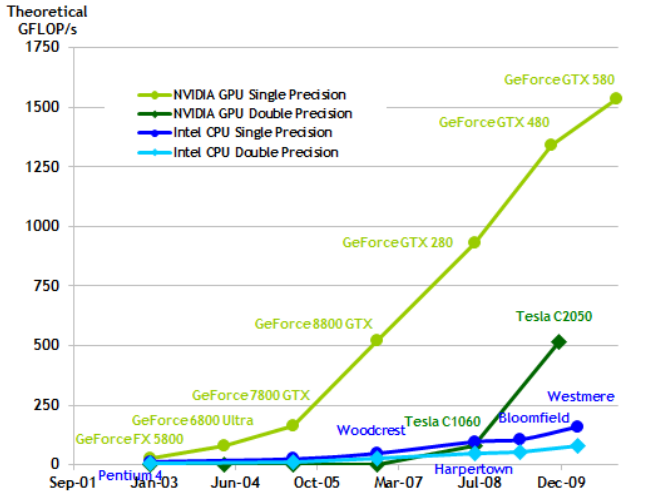
\includegraphics[scale=0.45]{images/cpuvsgpu.png}
\caption{GPU vs. CPU processor FLOPS performance gap.}
\label{fig:cpuvsgpu}
\end{figure}

In the other hand, the usage of graphical processor units have another important advantage over traditionally computing CPU based model; its memory bandwidth. In the last decade the gap between CPU and memory speed have kept growing, and thus memory latency has become a major bottleneck in CPU computing, specially in applications with an intensive usage of memory. The evolution of theoretical single precision floating point operations (FLOPS) for both Intel based CPU processors and NVIDIA based GPU processors is shown in the figure \ref{fig:cpuvsgpu}. 

First attempts of using GPUs with other purposes rather than graphics, required to transform or convert complex algorithms and data into a graphics, to be able to use the GPU through graphics libraries (like OpenGL) to solve them and later revert the transformation. 

NVIDIA, conscious that GPGPU could be an important boost for the GPU market and also knowing that the current approaches for using GPUs for general purpose programming required a high level of knowledge and was a tedious job, started developing an SDK with the purpose of simplifying the task of GPGPU programming. The result of this development was CUDATM (Compute Unified Device Architecture), that was launched in November 2006. 

CUDA is a parallel computing architecture that enables programmers to use both CPU and GPU processors to cooperate in a single program, using a computing paradigm known as heterogeneous computing. Software developers are able to program general purpose functions or routines to be run on the GPU by simply use “C for CUDA” (C with NVIDIA extensions) while the rest of the program is still executed in the CPU. 

CUDA has become widely used in many areas such as physics simulations, scientific and medical simulations, signal processing, cryptography or audio and video processing among others. ATI also launched his own GPGPU SDK called Stream SDK, but at the time Stream SDK has not been as successful as CUDA.

\subsection{CUDA architecture and programming model for GPGPU.}

The CUDA SDK allows programmers to code parts or functions of a general purpose program to be executed in the GPU using C language with some extensions. The main three key abstractions that are exposed to the programmer as the C extensions are: a hierarchy of thread groups, shared memories and thread barrier synchronization. CUDA programmers have to partition the algorithms or parts of the code that are going to be boosted using the GPU into coarse sub-problems that can be solved independently in parallel, and then into smaller pieces that can be solved cooperatively in parallel. Functions executed into the GPU are called kernels, the rest of the code, and particularly
high control intensive parts of the code, are executed on the CPU. 

\begin{figure}[h]
\centering
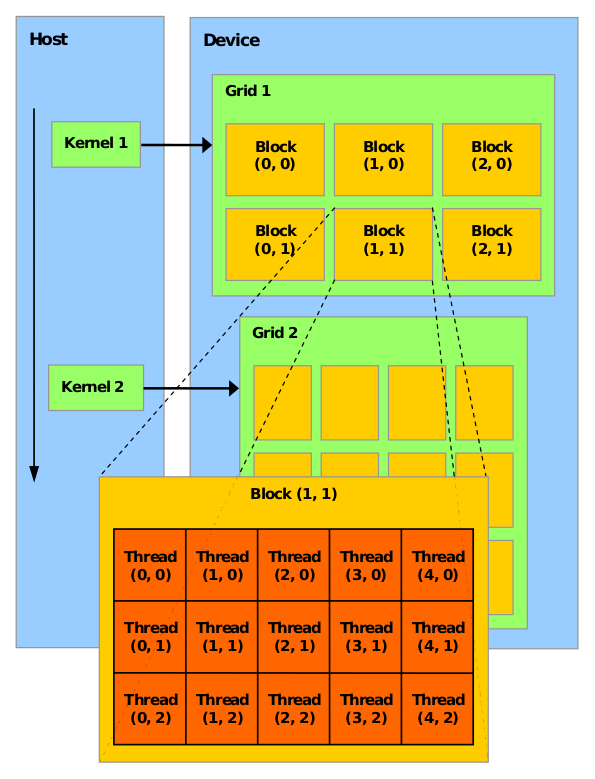
\includegraphics[scale=0.45]{images/cuda_threads.png}
\caption{CUDA thread hierarchy.}
\label{fig:cuda_threads}
\end{figure}

Kernels are functions designated with \_global\_ attribute. When they are called, kernels throw a total number of N threads. To achieve a good performance in general, kernels should throw thousands of threads. 

Figure \ref{fig:cuda_threads} show kernel’s thread organization of model. The N threads thrown by the kernel are organized in 2D array of blocks called grid, each of this blocks containing a 3D array of threads (hardware supports only 2D array at this moment). The number of threads, and their organization cannot be modified during the kernel execution. The programmer may use or not multidimensional block and grid organization according to their needs, simply not using (0 value) the dimensions not needed. 

The programmer can access to the current thread block ID dimensions values with variables blockIdx.x and blockIdx.y respectively. Likewise, the programmer can access to current thread ID dimension with variables threadIdx.x, threadIdx.y and threadIdx.z respectively. The combination of blockIdx and threadIdx complex variables values identify unequivocally each thread, and are used to perform ordered data accesses and execute code conditionally depending on the thread and block IDs. Currently, CUDA based programs have the restriction of a maximum of 65536 (216) threads and the limitation of 512 threads/blocks per dimension due to current GPU architectures (Tesla architecture).

\begin{figure}[h]
\begin{lstlisting}
__global__ void vecAdd (float *A , float *B , float *C)
{
	int i = threadIdx.x;
	C[i] = A[i] + B[i];
}

int main (int argc, char *argv[])
{
	vecAdd<<<Nb,Nt>>>(A, B, C);
	return 0;
}

\end{lstlisting}
\caption{Simplified CUDA kernel and associated main() function.}
\label{fig:cuda_threads}
\end{figure}

The code contained in the figure 2.12 shows a simplified example of a kernel call, throwing vecAdd kernel with a 1D grid organization and 1D thread block organization, throwing NB blocks, with NT threads per block. Some coding details, like memory data transfers from CPU to host are omitted for simplicity.


\setsecnumdepth{all}
\chapter{Design}
\label{chap:design}

\section{Developing tools and methodology.}
The tools and programming languages selected for implementing application are:

Languages:

\begin{itemize}
\item \textbf{C++}: due to perfomance requirements and supporting of object oriented features (classes, inheritance), C++ is used for developing the whole program, instead of the CUDA device code part, where C dialect for CUDA is used.
\item \textbf{CUDA}: CUDA uses C language with additional features to perform general purpose calculations in the GPUs.
\end{itemize}

Libraries:

\begin{itemize}
\item \textbf{Libpcap}: is packet-capture library for retrieving packets from the Packet Filter.
\item \textbf{QT}: is a cross-platform application framework for developing application with a rich graphical interface. It is used for building GUI part of the application.
\item \textbf{Boost}: is a set of libraries that extend the functionality of the C++ programming language. From boost libraries components for processes synchronization were used (semaphores and mutexes). Also boost.spirit parser is used to parse rules dataset.
\item \textbf{Sqlite}: is a software library that implements a SQL database engine and is used to store results.
\end{itemize}

The methodology used has been the spiral model.
\begin{figure}[h]
\centering
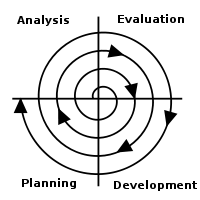
\includegraphics[scale=0.7]{images/spiral-model.png}
\caption{Spiral methodology used in the developing process of the application.}
\end{figure}

In this methodology, the process of determining requirements, analyzing possible risks, implementing, testing and planning (results evaluation), are performed during the whole project. The number of rotating through the spiral depend on the found implementation issues, the precision of objective definition in the early stages of the development and the requirements accomplishment of the current implementation.

\section{NIDS rules.}
NIDS rules dataset has a simple text format. Each line of the text file contain rule in the following format:


\begin{figure}[h]
\centering
\begin{verbatim}
action protocol src_ip src_port direction dst_ip dst_port {options}
\end{verbatim}
\caption{Rule format.}
\label{fig:rule_format}
\end{figure}

\textbf{Action} could be an \textbf{alert} or \textbf{log}, where 'alert' means that if case rule is matched against some packet it should be alerted to user, for example highlighted with a red color in a GUI. If rule starts with a 'log' action it means that packet matched against rule will be logged into a database without any specific actions for gaining user attention.

\textbf{Protocol} is a packet's protocol type. Because of simplifications only 'tcp' is supported by developing application.

\textbf{Src\_ip} is a source IP address of the packet. IP address is written in a standard form '192.168.0.1' where each position could be a range, for example '192.168.0-20.1'. Also instead of any position in the IP address, '*' symbol could be used to accept all values on that position. For example '192.168.*.*'.

\textbf{Src\_port} is a source TCP port. It is a value from 0 to 65535, or range, for example 5-1234, or '*' symbol which means any port.

\textbf{Direction} is a string "\textendash\textgreater". At this moment only this direction string is supported.

\textbf{Dst\_ip} is a destination IP address written in the same format as source IP address.

\textbf{Dst\_port} is a destination TCP port written in the same format as a source TCP port.

\textbf{Options} are parameters that specifies payload analysis. Within options should be a \textbf{content} or \textbf{pcre}. Content specifies a string which is searched within a packet payload. Also content string could contain raw bytes which should be written within '\textbar' symbols. Example of the content option with a string and raw bytes \textbf{content:"searchedstring\textbar00 01 02\textbar"}.\newline Pcre specifies the searched string as a regular expression. Example of pcre option \textbf{pcre:"\textasciicircum(some)*regex"}. The reason of dividing searched string on content and pcre is that all content strings are compiled into one DFA while each pcre is compiled in its own DFA and could consume much more memory. Options may contain parameters \textbf{offset} and \textbf{length} which means position in a payload from which searching should be started and number of bytes from the start position to observe. And finally \textbf{msg} parameter could be withing options. It is a simple string that should be logged or alerted to user when some packet matches against the rule.

\section{Application design overview.}
The main objective of this thesis is to design and implement simple NIDS application capable to analyze network traffic using GPUs, specifically using CUDA. 
\subsection*{Pattern matching.}
Pattern matching is the most heavy operation that affects the NIDS perfomance. Pattern matching algorithms can be classified into single-pattern and multi-pattern algorithms.

Single-pattern algorithms work in a way that each pattern is searched in a given text individually. Therefore for k searched patterns algorithm should be repeated k times. Some of the widely used algorithms are Knuth-Morris-Pratt and Boyer-Moore. Knuth-Morris-Pratt is able to skip characters when a mismatch occurs in the comparison phase using a partial match table for each pattern. Each table is built by preprocessing every pattern separately. Boyer-Moore is the most widely used single-pattern algorithm. Its execution time can be sublinear if the suffix of the string to be searched for appears infrequently in the input stream, due to the skipping heuristics that it uses.

Multi-pattern matching algorithms search a set of patterns in a text simultaneously. It is done by preprocessing all patterns that could be searched into an automation which is used during searching phase. The automation may be represented as a trie, a table or combination of the two. Such algorithms searches each byte from the text only once. Also such algorithms scales much better that single-pattern. Example of multi-pattern algorithms: Aho-Corasick, Wu-Manber and Commentz-Walter.

Previous section introduced NIDS rule which could contain \textbf{content} or \textbf{pcre} patterns that should be searched withing payload. As there could be a lot of rules and a lot of contents it was decided to use Aho-Corasick algorithm to search all content string simultaneously within packet payload. 

The Aho-Corasick algorithm consists of two parts. In the first part we construct from the set of patterns a finiste state machine; in the second part we apply the packet payload as input to the pattern matching machine. The machine signals whenever it has found a match for a keyword. The pattern matching machine consists of a set of states. Each state is represented by a number. The machine processes the text by successively reading symbols from input string, making state transitions and occasionally emitting output. The behaviour of the pattern matching machine is dictated by three functions: a goto function \emph{g}, a failure function \emph{f} and an output function \emph{output}. Figures \ref{fig:goto_function}, \ref{fig:failure_function} and \ref{fig:output_function} shows the functions used by a pattern matching machine for a set of keywords (he, she, his, hers).

\begin{figure}[h]
\centering
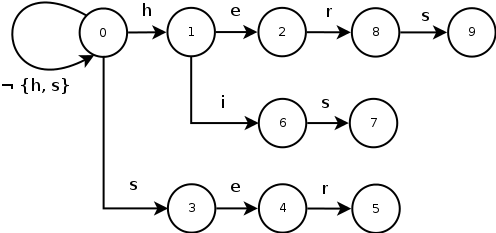
\includegraphics[scale=0.5]{images/goto_function.png}
\caption{Aho-Corasick goto function.}
\label{fig:goto_function}
\end{figure}

\begin{figure}[h]
\centering
\begin{tabular}{l l l l l l l l l l}
\emph{i}       & 1 & 2 & 3 & 4 & 5 & 6 & 7 & 8 & 9 \\
\emph{f(i)}    & 0 & 0 & 0 & 1 & 2 & 0 & 3 & 0 & 3 \\
\end{tabular}
\caption{Aho-Corasick failure function.}
\label{fig:failure_function}
\end{figure}

\begin{figure}[h]
\centering
\begin{tabular}{l l}
\emph{i} & \emph{output(i)} \\
2 & {he} \\
5 & {she, he} \\
7 & {his} \\
9 & {hers} \\
\end{tabular}
\caption{Aho-Corasick output function.}
\label{fig:output_function}
\end{figure}

One state (usually 0) is designated as a start state. In figure \ref{fig:goto_function} the states are 0, 1,...,9. The goto function \emph{g} maps a pair consisting of state and an input symbol into a state or the message fail. The directed graph in figure \ref{fig:goto_function} represents the goto function. The absence of an arrow indicates \emph{fail}. Thus, g(1, \emph{s}) = \emph{fail} for all input symbols \emph{s} that are not 'e' or 'i'.

The failure function \emph{f} maps a state into a state. The failure function is consulted whenever the goto function reports \emph{fail}. Certain states are designated as output states which indicate that a set of keywords has been found.

An operating cycle of a pattern matching machine is defined as follows. Let s be the current state of the machine and a the current symbol of the input string x.
\begin{enumerate}
\item If \emph{g(s, a) = s'}, the machine makes a goto transition. It enters state s' and the next symbol of x becomes the current input symbol.
In addition, if  \emph{output(s')  empty}, then the machine emits the set \emph{output(s')} along with the position of the current input symbol. The operating cycle is now complete.
\item If \emph{g(s, a) = fail}, the machine consults the failure function \emph{f} and is said to make a \emph{failure} transition. If \emph{f(s)=s'} the machine repeats the cycle with s' as the current state and a as the current input symbol.
\end{enumerate}
Initially, the current state of the machine is the start and the first symbol of the text string is the current input symbol. 

\begin{figure}[h]
\textbf{Input.} A text string $x = a_1 a_2 ... a_n$ where each $a_i$ is an input symbol and a pattern matching machine M with goto function \emph{g}, failure function \emph{f}, and output function \emph{output}.\\
\textbf{Output.} Locations at which keywords occur in x.\\
\textbf{Method.}
\begin{algorithmic}
\STATE $state \leftarrow 0$
\FOR{$i=1$ to $n$}
\WHILE{$g(state, a_i) = fail$}
\STATE $state \leftarrow f(state)$
\ENDWHILE
\STATE $state \leftarrow g(state, a_i)$
\IF{$output(state) \neq empty$}
\PRINT i
\PRINT $output(state)$
\ENDIF
\ENDFOR
\end{algorithmic}
\caption{Aho-Corasick pattern matching machine algorithm.}
\label{fig:ac_search_pseudocode}
\end{figure}

\begin{figure}[h]
\textbf{Input.} Set of keywords K={$y_1$, $y_2$,..., $y_k$} \\
\textbf{Output.} Goto function \emph{g} and a partially computed output function \emph{output}.\\
\textbf{Method.} We assume \emph{output(s)} is empty when state s is first created, and \emph{g{s, a} = fail} if \emph{a} is undefined or if \emph{g(s, a)} has not yet been defined. The procedure \emph{enter(y)} inserts into goto graph a path that spells out \emph{y}.
\begin{algorithmic}
\PRINT here will be algorithm
\end{algorithmic}
\caption{Aho-Corasick goto function construction algorithm.}
\label{fig:ac_goto_pseudocode}
\end{figure}

\begin{figure}[h]
\textbf{Input.} Set of keywords K={$y_1$, $y_2$,..., $y_k$} \\
\textbf{Output.} Goto function \emph{g} and a partially computed output function \emph{output}.\\
\textbf{Method.} We assume \emph{output(s)} is empty when state s is first created, and \emph{g{s, a} = fail} if \emph{a} is undefined or if \emph{g(s, a)} has not yet been defined. The procedure \emph{enter(y)} inserts into goto graph a path that spells out \emph{y}.
\begin{algorithmic}
\PRINT here will be algorithm
\end{algorithmic}
\caption{Aho-Corasick fail function construction algorithm.}
\label{fig:ac_fail_pseudocode}
\end{figure}

Figure \ref{fig:ac_search_pseudocode} shows Aho-Corasick matching machine algorithm pseudocode. Pseudocodes for construction of \textbf{Goto}, \textbf{Failure}, and \textbf{Output} are shown in figures \ref{fig:ac_goto_pseudocode} and \ref{fig:ac_fail_pseudocode}.

\begin{figure}[h]
\textbf{Input.} Set of keywords K={$y_1$, $y_2$,..., $y_k$} \\
\textbf{Output.} Goto function \emph{g} and a partially computed output function \emph{output}.\\
\textbf{Method.} We assume \emph{output(s)} is empty when state s is first created, and \emph{g{s, a} = fail} if \emph{a} is undefined or if \emph{g(s, a)} has not yet been defined. The procedure \emph{enter(y)} inserts into goto graph a path that spells out \emph{y}.
\begin{algorithmic}
\PRINT here will be algorithm
\end{algorithmic}
\caption{Aho-Corasick DFA construction algorithm.}
\label{fig:ac_dfa_pseudocode}
\end{figure}

To be able to use Aho-Corasick algorithm with a GPU a DFA should be constructed from the previously constructed \textbf{Goto}, \textbf{Fail} and \textbf{Output} functions. The algorithm for constructing DFA is shown in a figure \ref{fig:ac_dfa_pseudocode}. In practice, algorithm shown in figure \ref{fig:ac_dfa_pseudocode} should be evaluated in conjunction with algorithm \ref{fig:ac_fail_pseudocode}. The resulting DFA is a two dimensional array. The dimensions of the array are equal to the number of states and the size of the alphabet (256 in our case) plus one position to store flag if state is \emph{output}.

The algorithm for searching through DFA is similar to the regular expression's one and described in the next section.

\subsection*{Regular expression pattern matching.}
Regular expressions are compiled into a DFA by using external library. As a result a two dimensional array is obtained. Array structure is similar to Aho-Corasick DFA. The dimensions of the array are equal to the number of states and the size of the alphabet (256 in our case) plus one position to store index of the rule if current state signs that regular expression is matched. Therefore the final algorithm for searching pattern withing packet payload is shown in figure \ref{fig:dfa_search}.

\begin{figure}[h]
\textbf{Input.} Set of keywords K={$y_1$, $y_2$,..., $y_k$} \\
\textbf{Output.} Goto function \emph{g} and a partially computed output function \emph{output}.\\
\textbf{Method.} We assume \emph{output(s)} is empty when state s is first created, and \emph{g{s, a} = fail} if \emph{a} is undefined or if \emph{g(s, a)} has not yet been defined. The procedure \emph{enter(y)} inserts into goto graph a path that spells out \emph{y}.
\begin{algorithmic}
\PRINT here will be algorithm
\end{algorithmic}
\caption{Pattern matching DFA search.}
\label{fig:dfa_search}
\end{figure}

\subsection*{Packet filtering based on route information.}
Information obtained from packet header is used to select packet for analysing its payload or drop it without any analysis. Information from loaded rules should match the packet's header information to continue processing of received packet. It was decided to store route information from the loaded rule as a sequence of bytes in a trie structure. Figure \ref{fig:trie_example} shows example of a trie structure with next IP addresses stored: 192.168.0.1, 192.168.1.38, 192.168.5-100.1 and 232.222.1.79. The full sequence stored in trie is shown in a figure \ref{fig:route_sequence}. Theresore to compare any received packet to some rule, route information from packet's header should be represented as a sequence of bytes shown in a figure \ref{fig:route_sequence}, and search procedure on a trie for the sequence of bytes is perfomed. This approach is similar to Aho-Corasick algorithm of searching with data saved in trie. The only difference is that trie may contain IP range (therefore trie node may be not just a simple node with value, but contain range of values). If search in trie found any rule for this packet, this packet is put in a queue for a payload analysis. 

\begin{figure}[h]
\centering
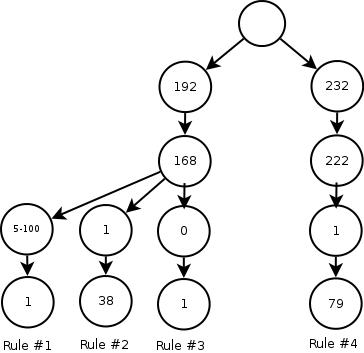
\includegraphics[scale=0.6]{images/trie.png}
\caption{Example of trie structure.}
\label{fig:trie_example}
\end{figure}

\begin{figure}[h]
\centering
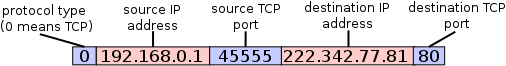
\includegraphics[scale=0.8]{images/route_sequence.png}
\caption{Full route sequence extracted from packet header.}
\label{fig:route_sequence}
\end{figure}

\subsection*{Transfering packets to the GPU.}
The simplest approach is to transfer each packet to the GPU separately. However, there is an overhead associated with a data transfer operation to the GPU and many small transfers to the GPU result into a perfomance decreasing. Therefore the following approach is designed to achieve better perfomance for packets transfering. Packets obtained by CPU are collected in a buffer for some time. When CPU decides that it's time to process packets it transfers a batch of packets to the GPU for processing. 

CPU program decision on transferring packets to the GPU could be based on two policies:
\begin{itemize}
\item Decision based on the time. Buffer with packets is transfered to the GPU on timer event.
\item Decision based on buffer size. Buffer with packets is transfered to the GPU when size of the buffer exceeds some size.
\end{itemize}

\subsection*{Database structure.}

\begin{figure}[h]
\centering
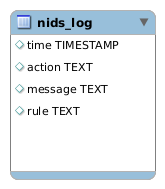
\includegraphics[scale=0.55]{images/database.png}
\caption{Database structure.}
\label{fig:database_structure}
\end{figure}

Database with results is very simple and contain only one table which have all information about matched packet inside. Figure \ref{fig:database_structure} shows table fields that are filled for a matched packets.
\begin{itemize}
\item \textbf{Time} field contains timestamp when NIDS detected suspicious packet.
\item \textbf{Action} field contains action from the matched rule.
\item \textbf{Message} field contains message from the matched rule.
\item \textbf{Rule} field contains the matched rule itself.
\end{itemize}
In the current application version it was decided not to save payload from the matched packet because of perfomance reasons.

\subsection*{Application components.}
Application design is divided into a several components. The diagram contained in a figure \ref{fig:app_architecture} shows the relationship between components.

\begin{figure}[h]
\centering
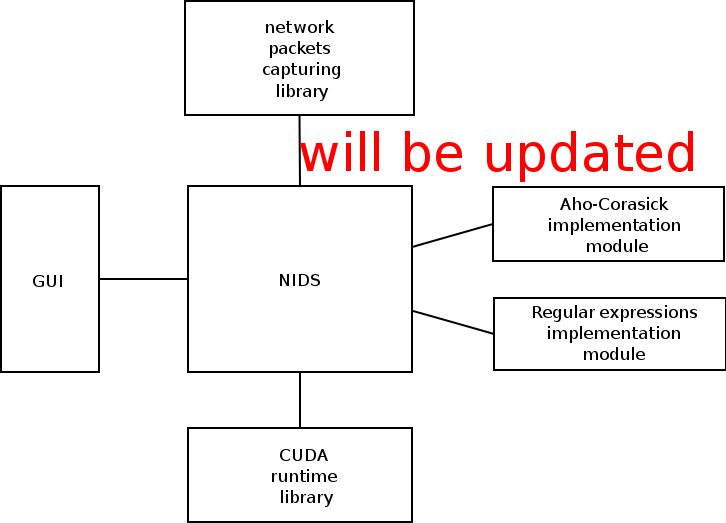
\includegraphics[scale=0.5]{images/app_architecture.png}
\caption{Relation between application components.}
\label{fig:app_architecture}
\end{figure}

\begin{itemize}
\item \textbf{GUI}. Component which implements user interactions with a program. Application has simple window-based interface which allows to perform all major manipulations with the application like starting capturing traffic, stop capturing, switching analyzing mode, saving traffic into the file, etc.
\item \textbf{Network packets capturing library}. Application itself doesn't capture packet from the kernel, because it is not a trivial task. Instead, program uses external library for packet capturing.
\item \textbf{NIDS}. The main component of the system. Uses all others modules to read rules, start capturing and analysing of packets. Stores results of analyzing into a database and updates counters which are used within NIDS to do perfomance calculations.
\item \textbf{Regular expressions implementation}. This module is used to compile regular expression obtained from rules. Regular expressions are compiled to DFA for loading into CUDA device later.
\item \textbf{Aho-Corasick implementation}. This module is used to create DFA for all simple content strings that are read from rules. Application uses Aho-Corasick algorithm for fast string searching within network packets.
\item \textbf{CUDA module}. Code that runs on a GPU and performs analysis of packets against rules.
\item \textbf{Database module}. Used for logging matched packets into the database.
\end{itemize}

\chapter{Implementation.}
\section{General considerations.}
Application implementation has been developed using the following version of the programming tools and libraries:
\begin{itemize}
\item GCC 4.7.0.
\item CUDA [TODO:add version]
\item LibPcap [TODO:add version]
\item QT [TODO:add version]
\end{itemize}

\lstset{language=Python, caption={Part of QT project file with extra compiler configuration.}, label=lst:extra_compiler_config, captionpos=b}
\begin{lstlisting}
# CUDA settings (for Arch Linux)
CUDA_SOURCES += my_nids_cuda.cu
# Path to cuda toolkit install
CUDA_DIR = /opt/cuda-toolkit
# GPU architecture
CUDA_ARCH = sm_11
# nvcc flags (ptxas option verbose is always useful)
NVCCFLAGS = --compiler-options -fno-strict-aliasing -use_fast_math --ptxas-options=-v
# include path
INCLUDEPATH += $$CUDA_DIR/include
# lib dir
QMAKE_LIBDIR += $$CUDA_DIR/lib64
# libs
LIBS += -lcudart
# join the includes in a line
CUDA_INC = $$join(INCLUDEPATH,' -I', '-I', ' ')

# Prepare the extra compiler configuration (taken from the nvidia forum)
cuda.input = CUDA_SOURCES
cuda.output = ${OBJECTS_DIR}${QMAKE_FILE_BASE}.o
cuda.commands = $$CUDA_DIR/bin/nvcc -m64 -g -G -arch=$$CUDA_ARCH -c $$NVCCFLAGS $$CUDA_INC $$LIBS ${QMAKE_FILE_NAME} -o ${QMAKE_FILE_OUT}

cuda.dependcy_type = TYPE_C
cuda.depend_command = $$CUDA_DIR/bin/nvcc -g -G -M $$CUDA_INC $$NVCCFLAGS ${QMAKE_FILE_NAME}
# Tell Qt that we want add more stuff to the Makefile
QMAKE_EXTRA_COMPILERS += cuda
\end{lstlisting}

The NIDS application has been developed based on the design presented in the chapter \ref{chap:design}. The application uses workflow presented in \ref{}. Project sources are organized into QT project file and to compile project first qmake utility from QT is used to generate Makefile. Makefile is required by \textbf{make } utility to compile and link sources into final executable. The whole project structure is placed in one folder, but logically source codes are divided into "Headers", "Sources", "Forms" and "Other files" if IDE such as QT creator is used to manage a project. All source codes are compiled with \textbf{gcc} compiler except CUDA code. Files with CUDA source codes have \textbf{*.cu} extension and are compiled with \textbf{nvcc} compiler. To add possibility to compile \textbf{*.cu} files to QT project an extra compiler configuration is created in QT project file (shown in listing \ref{lst:extra_compiler_config}).

\section{Application threading model.}
The NDIS application has been developed using Boost.Thread library for Nids itself and QThread for GUI part. Boost.Thread is used in the main Nids class for processing packets on CPU or GPU. The QThread is used for executing Main window message processing and running Nids packet capture task. The reason why two different threads classes were used is that developing of the core Nids application was started using only Boost library and QT part is added a little bit later.

When NIDS application process in CPU mode N threads are created for packet processing and 1 thread is created for packets collecting. Packet capture thread writes packet payload into a buffer and puts pointer to the buffer into a queue. Other threads are sleep until some packet arrive in the queue. In the moment when packet arrived in the queue one of the thread awakes and pulls packet from the queue for processing. After finishing working on packet it goes to sleep state again until new packet arrive into the queue.

For NIDS working in CPU+GPU mode packets processing is slightly different. There is only 1 thread which puts tasks (packet payload, payload length and number of DFA to search) into the queue and 1 thread which process packets when size of the packets in the queue exceeds threshold or time for processing elapsed. A double-buffered mechanism of processing packets were implemented to speed up the process of collecting packets: before processing packets on GPU buffers are switched and CPU is able to collect arriving packets into the second buffer.

To keep multithreaded code integrity, synchronization mechanisms from Boost library were used: Boost.Semaphore for synchronizing access to queues and Boost.Mutex for synchronizing access to other objects.

\begin{figure}
\centering
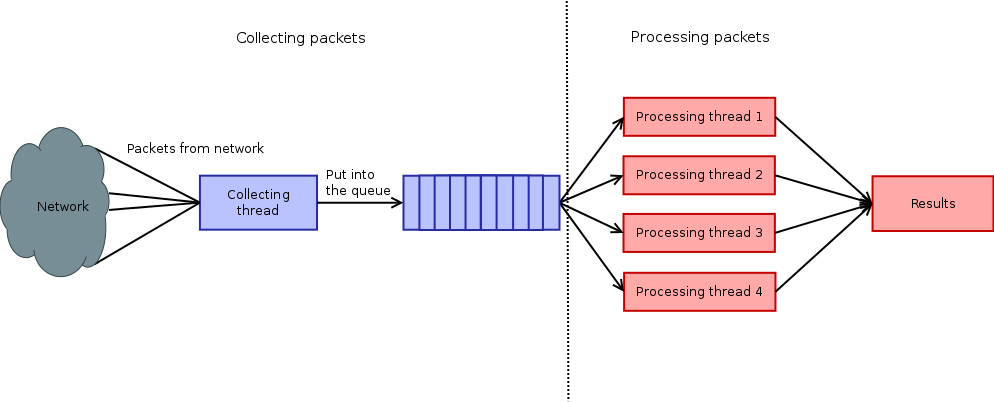
\includegraphics[scale=0.3]{images/cpu_threads.png}
\caption{Threading model for CPU processing.}
\label{fig:cpu_threads}
\end{figure}

\begin{figure}
\centering
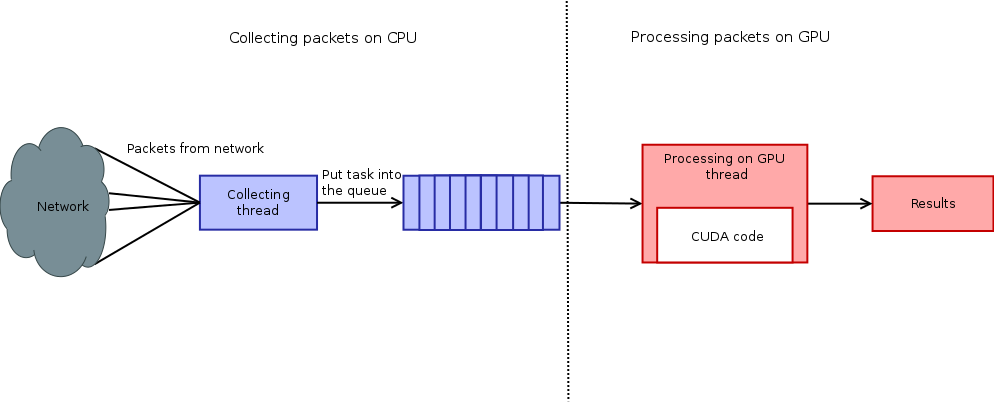
\includegraphics[scale=0.3]{images/gpu_threads.png}
\caption{Threading model for CPU+GPU processing.}
\label{fig:gpu_threads}
\end{figure}

Figures \ref{fig:cpu_threads} and \ref{fig:gpu_threads} shows the threading model for CPU and CPU+GPU modes graphically.

\section{Main application classes.}
In this section the main application classes are described, their functionality and purpose.

\subsection{Packet class.}
Packet class is used to store all information about network packet needed to analyze packet header and payload. It is used by Nids class to search within trie structure and analyze payload for regex or ac patterns. Listing \ref{lst:packet_class} shows part of the implementation of the class header.

\lstset{language=C++, caption={Extract of Packet.h}, label=lst:packet_class, captionpos=b}
\begin{lstlisting}
class Packet
{
public:
    Packet(in_addr ip_from, in_addr ip_to, int port_from, int port_to);

    // create packet from raw data
    static Packet* create_packet(const u_char *raw_packet);

    // for test purposes
    static Packet* create_fake_packet();

    // getters and setters for packet components
    in_addr get_ip_from() const;
    // ...

    sequence32 &get_route();
    const sequence32 &get_route() const;
    int get_payload_offset() const;
    int get_payload_size() const;
    const u_char *get_raw_packet() const;

    // payload from raw_packet is saved into internal vector
    // it means that packet will be analyzed by CPU
    vector<u_char> &save_payload();
    const vector<u_char> &get_payload() const;

private:
    //...
    int payload_size;
    int payload_offset;

    // info about route for analyzing in the trie
    sequence32 route;
    const u_char *raw_packet;
    vector<u_char> payload;
};
\end{lstlisting}

When new packet is arrived a create\_packet static method is used to analyze packet. This method is a packet analyzer and it's used for every received packet to create Packet class with properly filled fields. Method create\_packet analyzes raw packet data and makes protocol identification. In case it is TCP/IP packet it creates Packet object, otherwise it returns null object which means that it's not needed to analyze received packet.

Right after returning from create\_packet method raw\_packet field contains the pointer to the raw packet payload. Method create\_packet doesn't copy payload data into any other place because of efficienty. This moment is described later in Nids class description.

Field route is used to save packet route information in the format described in figure \ref{fig:route_sequence}. The route information is stored in sequence32 type array which is defined as a std::vector class that contain 32 bit values. There is also sequence8 type in the application which is std::vector itself containing 8 bit values.

\subsection{AC class.}
AC class is the implementation of the Aho-Corasick algorithm. The main methods are insert and search. Method insert inserts some string into the internal trie and search tries to find given string within saved strings. When all strings are inserted finish method should be called to process all strings into a DFA which later can be extracted for loading to GPU. 

\lstset{language=C++, caption={Extract of AC.h}, label=lst:ac_class, captionpos=b}
\begin{lstlisting}
#define FAIL -1
#define STATE_SIZE UCHAR_MAX + 1

class AC
{
public:
    AC();

    void insert(const sequence8 &sequence, int value);
    void search(const sequence8 &sequence, vector<int> &result);
    void search(const u_char *sequence, int length, vector<int> &result);
    int next(int state, sequence_val8 value);

    void finish();
    int count_states();
    int get_transition_value(int state, int c);
    const vector<int> &get_transition_row(int state);
    const vector<int> &get_out(int state);

private:
    void enter(const sequence8 &sequence, int value);
    void compute_fail_transitions();

    vector< vector<int> > transition_table;
    vector< vector<int> > out;
};
\end{lstlisting}

Internally DFA is stored in a transition\_table field with unbounded maximum number of states and number of transitions for the state equals to UCHAR\_MAX + 1 (256). Field out is an out function as described in Aho-Corasick algorithm description. For every state it contains all matched strings.

\begin{figure}[h]
\centering
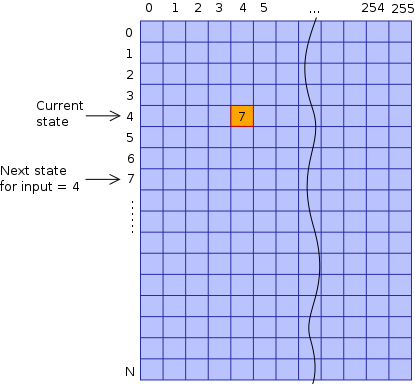
\includegraphics[scale=0.5]{images/ac_grid.png}
\caption{Aho-Corasick DFA traversing.}
\label{fig:ac_grid}
\end{figure}

The search algorithm is simple traversing internal DFA for every next input symbol is shown on figure \ref{fig:ac_grid}.

\subsection{Regex class.}
Regex class implements compilation of regex patterns into DFA and searching in the input strings for previously compiled patterns. The main methods are compile and search. 

\lstset{language=C++, label=lst:regex_class, captionpos=b, caption={Extract of Regex.h}}
\begin{lstlisting}
#define STATE_SIZE (UCHAR_MAX + 1)
#define STATE_DEAD -1
#define STATE_WHOLE_STR -2

class Regex
{
public:
    Regex();

    int compile(const sequence8 &regex);
    int count_states();
    int get_transition_value(int dfa_offset, int state, int c);
    const vector<int> get_transition_state(int dfa_offset, int state);
    const vector<int> get_transition_state(int row);
    bool is_match(int dfa_offset, int state);
    bool is_match(int row);
    const vector<int> get_dfa_offsets() const;
    bool search(const sequence8 &data, int dfa_offset);
    bool search(const u_char *data, int length, int dfa_offset);

private:
    vector< vector<int> > transition_table;
    vector<int> dfa_offsets;
    int states_total;
    int states_cur_dfa;
    map<void *, int> states_map;
    const re2::uint8 *bytemap;

    int analyze_state(void *state);
};
\end{lstlisting}

Method compile uses RE2 regular expression library to compile input pattern into DFA. Default memory budget for compiling one DFA is 8388608 bytes. If compiling pattern exceed memory budget such regex is declined and won't be searched during packet analyzing.

\begin{figure}[h]
\centering
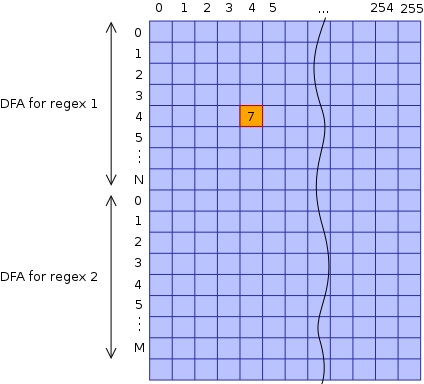
\includegraphics[scale=0.5]{images/regex_grid.png}
\caption{Regex DFA internal representation.}
\label{fig:regex_grid}
\end{figure}

The internal representation of DFA is similar to AC's one. The only difference is that AC has one DFA and all input string falls into it, while for every regular expression separate DFA is created. Thus, Regex class stores all DFAs into one vector and to be able to find specific DFA start offsets are stored into other vector. Other difference is that regex DFA contains states defined as STATE\_DEAD and STATE\_WHOLE\_STR. This states finish the whole searching procedure: value STATE\_DEAD means that for any input character the next state is the current one, value STATE\_WHOLE\_STR means that no matter what next input symbols could be, current searching procedure in any case cannot succeed (e.g. searched pattern should match from the start of the string, if start is not matched, not matter what are the other symbols, searching could not succeed).
Regex DFAs representation stored in Regex class is shown in figure \ref{fig:regex_grid}.

\subsection{Trie class.}
Trie class is used to store the sequence of symbols and quick search over the input string. Internal structure of the trie was described in \ref{TODO:add ref}. Trie class itself contain only three methods: insert, search and clear. The name of the methods are pretty clear and speaks for themselfs.

\lstset{language=C++, label=lst:trie_node_class, captionpos=b, caption={Extract of Trie_node.h}}
\begin{lstlisting}
typedef vector<trie_range> trie_range_t;
typedef vector<Trie_node *> trie_range_value_t;
typedef map<sequence_val32, Trie_node *> trie_transition_t;

class Trie_node
{
public:
    Trie_node();
    vector<int>& get_values();
    void set_values(vector<int> &values);
    void append_values(vector<int> &values);
    void append_value(int value);
    Trie_node *next(sequence_val32 val);
    void set_next(sequence_val32 val, Trie_node *next);
    void set_next_any(Trie_node *next);
    Trie_node *get_next_any();

    trie_transition_t &get_transitions();
    trie_range_t &get_ranges();
    trie_range_value_t &get_range_values();

private:
    trie_transition_t next_;
    trie_range_t range_next_;
    trie_range_value_t range_next_value_;
    Trie_node *any_next_;
    vector<int> values;
};
\end{lstlisting}

More complex is the Trie\_node class which stores information for one trie node (listing \ref{lst:trie_node_class}). The type trie\_transition\_t maps symbol value to the next trie node. Thus the search algorithm is similar to the searching over DFA, but trie node additionally contains range\_next\_ field which is used to store range for IP or port values. If, for example, 192.0-4.*.* is used, than range\_next\_ will contain 0-4 part of the IP address in current trie node. Also any\_next\_ is the pointer to the next trie node, so for * symbol used in IP address any\_next\_ field is filled with pointer to the next trie node. Therefore searching over such kind of the trie is getting next trie node from the next\_ field for each input symbol from the input string. Additionally check if range or any symbol exist in the current node.

\subsection{Rule class.}
For each rule in the rules.txt file one object of Rule class type is created. Rule class stores a text representation of the rule and also all parameters of the rule which are parsed by using Boost.Spirit parser.

\lstset{language=C++, label=lst:rule_class, captionpos=b, caption={Extract of Rule.h}}
\begin{lstlisting}
class Rule
{
public:
    static Rule *create_rule(const string &rule);

    Action get_action();
    const sequence32 &get_route();
    // ...

private:
    Rule();
    // ...

    // rule as string
    string rule_str;
    // action that should be taken if rule is matched
    Action action;
    // message that should be inserted into database if this rule matched
    string message;
    // route info includes all information about protocol and IP adresses and ports.
    // it will be inserted in trie and matched against route info of every received packet.
    sequence32 route;
    vector<sequence8> content;
    sequence8 pcre;
    int offset;
    int length;
};

\end{lstlisting}

The Rule object is created using static create\_rule method. This method simply parses passed string value and returns pointer to newly created Rule object with filled parameters. Parsing is done by using Boost.Spirit library which allows to write grammar for parsing directly in the C++ code. For parsing rules a RuleRouteGrammar was created and used in a Boost's phrase\_parse function. In case of malformed rule create\_rule function returns NULL. Listing \ref{lst:ip_grammar} contains an example of a simple grammar for parsing IP address. This grammar returns std::vector object with four ip parts represented as unsigned integers.

\lstset{language=C++, label=lst:ip_grammar, captionpos=b, caption={Boost.Spirit grammar for parsing IP address.}}
\begin{lstlisting}
template<typename Iterator>
struct IPGrammar : qi::grammar<Iterator, std::vector<unsigned>(), space_type>
{
    IPGrammar() : IPGrammar::base_type(ip_address)
    {
        ip_address = uint_parser<unsigned, 10, 1, 3>() >> '.' >> 
                     uint_parser<unsigned, 10, 1, 3>() >> '.' >> 
                     uint_parser<unsigned, 10, 1, 3>() >> '.' >> 
                     uint_parser<unsigned, 10, 1, 3>();
    }

    qi::rule<Iterator, std::vector<unsigned>()> ip_address;
}
\end{lstlisting}

Grammar could be easily extended to include new parameters by adding qi::rule as a field and include new rules definitions into IPGrammar. Boost.Spirit allows to parse strings directly into C++ structures, so it is possible to create structures layout for parsing very complex expressions.

\subsection{Nids class.}

Nids class is the main class in the application. It manages all activities in the application, starts and stops network monitoring, all previously described classes are used by Nids class as helpers. 

\lstset{language=C++, label=lst:nids_class, captionpos=b, caption={Extract of Nids.h}}
\begin{lstlisting}
class Nids
{
public:
    Nids();
    ~Nids();

    int read_rules(const char *filename);
    bool start_monitor(const char *interface, int threads_num, const char *db_filename = NULL);
    bool start_monitor_gpu(const char *interface,
                           int device_num,
                           WINDOW_TYPE window_type = BUF_SIZE,
                           int buf_threshold_size = DEF_PACKET_BUFFER_SIZE,
                           int buf_flush_time = DEF_TIME_FLUSH_BUFFER,
                           const char *db_filename = NULL);
    bool start_monitor_offline(const char *interface, 
                           const char *cap_filename, 
                           int threads_num, 
                           const char *db_filename = NULL);
    bool start_monitor_offline_gpu(const char *interface, 
                           const char *cap_filename, 
                           int device_num,
                           WINDOW_TYPE window_type = BUF_SIZE,
                           int buf_threshold_size = DEF_PACKET_BUFFER_SIZE,
                           int buf_flush_time = DEF_TIME_FLUSH_BUFFER,
                           const char *db_filename = NULL);
    bool start_monitor_dump(const char *interface, const char *cap_filename);
    // ...
    void add_alert_callback(AlertCallbackFunc callback, void *user);
    void add_log_callback(LogCallbackFunc callback, void *user);

private:
    // ...

    // loaded rules
    vector<Rule *> rules;

    // route info saved in trie
    Trie rules_trie;

    // ...

    // CPU processing
    // ...
    boost::interprocess::interprocess_semaphore packets_queue_sem;
    boost::interprocess::interprocess_semaphore threads_finished_sem;
    boost::interprocess::interprocess_semaphore process_result_sem;
    boost::interprocess::interprocess_mutex packets_queue_mutex;
    boost::interprocess::interprocess_mutex analyzing_result_mutex;

    // GPU processing
    // ...
    // pointers to current buffer that should be processed on gpu
    vector<int> *gpu_ac_rules;
    vector<u_char> *gpu_packet_buffer;
    vector<int> *gpu_tasks;

    // double buffered packets, tasks and ac_rules
    vector<int> ac_rules1;
    vector<int> ac_rules2;
    vector<u_char> packet_buffer1;
    vector<u_char> packet_buffer2;
    vector<int> tasks1;
    vector<int> tasks2;

    vector<int> analyze_rules;
    vector<int> matched_rules;

    // CUDA synchronization semaphores
    boost::interprocess::interprocess_semaphore gpu_task_ready;
    boost::interprocess::interprocess_semaphore gpu_task_finished;
    boost::interprocess::interprocess_semaphore gpu_init_finished;
    boost::interprocess::interprocess_mutex gpu_switch_buffer_mutex;

		void switch_buffers();
    // ...
    friend void packet_received(u_char *user, const struct pcap_pkthdr *h, const u_char *bytes);
    friend struct process_on_gpu_callable;
    friend struct process_on_cpu_callable;
    friend struct process_results_callable;
};\end{lstlisting}

When application is started it should read Nids rules first. For this process read\_rules method is used: it creates array of rules in a \textbf{rules} variable and uses these rules for packet analysis.

Different start\_* methods are used to start monitoring network in different modes:
\begin{itemize}
\item \textbf{start\_monitor} is used to start network monitoring in a CPU mode. Number of threads used to process packets is passed as threads\_num parameter.
\item \textbf{start\_monitor\_gpu} is used to start network monitoring in a CPU+GPU mode. Pararmeter window\_type specifies what kind of flush mechanism is used for transferring packets to GPU: BUF\_SIZE or TIME. Parameter device\_num specifies which GPU device is used for packets analyzing.
\item \textbf{start\_monitor\_offline} is used to process packets from saved *.cap file in CPU mode. It operates in the same manner as start\_monitor, the only difference that new parameter cap\_filename is used as a name of the file with packets.
\item \textbf{start\_monitor\_offline\_gpu} is used to process packets from saved *.cap file in CPU+GPU mode. It operates in the same manner as start\_monitor\_gou, the only difference that new parameter cap\_filename is used as a name of the file with packets.
\item \textbf{start\_monitor\_dump} is used to start monitoring network and save packets into the *.cap log file. Later this file is used by previously defined methods for analyzing.
\end{itemize}

Just after starting monitoring network Nids class creates threads for processing packets on CPU or GPU. For this purpose three process\_* structures were created:
\begin{itemize}
\item \textbf{process\_on\_gpu\_callable} is a structure with overrided operator (). This way Boost.Thread executes code in operator() in a separate thread. The process\_on\_gpu\_callable thread performs tasks execution on GPU. Because CUDA device should be initialized in the thread where it will be used, process\_on\_gpu\_callable also initializes CUDA device. For synchronization purposes during initialization and processing on GPU Boost.Semaphore and Boost.Mutex is used. For example, after Nids started process\_on\_gpu\_callable thread, it waits on gpu\_init\_finished semaphore until thread finishes initializing CUDA device.
\item \textbf{process\_on\_cpu\_callable} has similar structure with overrided operator (). Parameter threads\_num defines how many process\_on\_cpu\_callable threads will be created. Every process\_on\_cpu\_callable thread waits on packets\_queue\_sem until new packet appears in the queue. For every packet exactly one thread will seize the packets\_queue\_sem and get packet from the queue.
\item \textbf{process\_results\_callable} is a thread which process results of the analysis. The thread main task is to insert matched rules into a database. There are also mechanism of the callbacks in Nids class. Callbacks functions can be added to Nids using add\_alert\_callback or add\_log\_callback methods and for every matched rule process\_results\_callable thread will call it.
\end{itemize}

The \textbf{packet\_received} function is a callback for a pcap library. Pcap call this function every time the new packet arrived into the system. The main responsibility of this function in CPU mode is to check whether new packet is TCP/IP (using Packet::create\_packet() method), create the Packet class object and put it into the queue. For CPU+GPU mode processing of the received packet is slightly different. The Packet class object is created as it is done in CPU mode, but just after creation all parsed parameters are saved into internal vectors (including payload) and Packet object is deleted. This way Nids class gathers all payloads into the one linear buffer and if the buffer size exceeds limit it increases gpu\_task\_ready semaphore to awake process\_on\_gpu\_callable thread to process packets on the GPU. Also CPU+GPU mode manages \textbf{tasks} array. This array is directly copied to the CUDA device and contains tasks that CUDA threads will process. The structure of task is described later in the CUDA code description.

The Nids class has two vectors for CUDA tasks and packet buffer. This way double-buffered mechanism is implemented for packet capturing and CUDA processing. When process\_on\_gpu\_callable thread copies data to the GPU and executes kernel on \textbf{tasks1} vector of tasks, packet\_received adds newly received packets to the \textbf{tasks2} vector of tasks.

Nids class logs a lot of information during its work. To reduce logged information set\_log\_level method is used. It defines six different log levels, but the major ones are: TRACE, DEBUG and INFO.

\subsubsection*{Future work.}
The future work for the Nids class is to implement packet categorization based on the payload size and process different categories of packets separately. There could be several categories of packets: small, medium, large, etc. This way CUDA resources could be used more effectively.

\subsection{CUDA code.}
The code on the CUDA device is quite simple. It receives array of tasks, pointer to packets buffer and pointer to DFAs buffer. Every CUDA thread gets task from the tasks buffer which contain information about data for processing. The packet processing is just traversing over DFA table for every input byte from the packet payload. If new state is the final one and has \textbf{found} flag  set, CUDA thread sets \textbf{found} flag for the current task. The task structure is described in the figure \ref{fig:cuda_task}.

\begin{figure}[h]
\centering
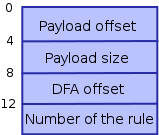
\includegraphics[scale=0.5]{images/cuda_task.png}
\caption{Cuda task.}
\label{fig:cuda_task}
\end{figure}

When CUDA kernel is starte, every CUDA thread calculates task using formula: \textbf{task\_num = blockIdx.x * blockDim.x + threadIdx.x}. This way every thread process takes task in sequential order. CUDA has limits on the number of threads per block (maximum 512 threads), but the number of tasks could be greather than the maximum number of threads, therefore CUDA code reuses threads to process all tasks. If we are using 4 block with 256 threads in each block, than maximum number of threads is 1024. This way only 1024 threads are logically executed in the same moment and should be reused for tasks that are not processed yet. The mechanism of thread resuing is described in the figure \ref{fig:cuda_thread_reuse}.

\lstset{language=C++, label=lst:nids_class, captionpos=b, caption={Extract of my\_nids\_cuda.cu}}
\begin{lstlisting}
    while (task_num < tasks) {
        // ...
        while (cur_idx < payload_length) {
            if (cache_index >= 64) {
                for (int i = 0; i < 16 && (cur_idx + i*4 < payload_length); ++i) {
                    payload_cache[i] = ((unsigned int*)(payload + cur_idx))[i];
                }
                cache_index = 0;
            }
            __syncthreads();

            if (cur_state == -1)
                break;

            if (cur_state == -2) {
                out_buffer[task_num] = result_rule;
                break;
            }

            if (dfa_state[256] > 0) {
                if (dfa_offset == dfa)
                    out_buffer[task_num] = cur_state;
                else
                    out_buffer[task_num] = result_rule;

                break;
            }

            cur_state = dfa_state[((unsigned char *)payload_cache)[cache_index]];
            ++cur_idx;
            ++cache_index;
        }

        // next task for the thread
        task_num += gridDim.x * blockDim.x;
    }
\end{lstlisting}

To speed up the process of analyzing packet on the GPU shared memory is used. Shared GPU memory has less access time than the global memory where all packets are situated. Each thread uses shared memory to copy small part of the payload for analyzing. When thread finishes analyzing part of the payload, it copies next part and so on until whole payload is analyzed. Application uses 64 bytes of a shared memory for each thread, because application mainly tested on Geforce 9600M GT which has 16Kb of shared memory per block.

\begin{figure}[h]
\centering
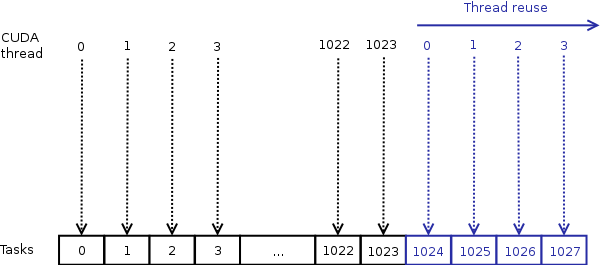
\includegraphics[scale=0.5]{images/cuda_thread_reuse.png}
\caption{Cuda threads reuse.}
\label{fig:cuda_thread_reuse}
\end{figure}

\subsubsection*{Future work.}
The future work for the CUDA code is to use texture memory to save DFA and\\or packets payload. Texture memory has the same access time as a global memory: 400-600 cycles. The only difference the Nids application is that texture memory is cached and in case of the cache hit access time is about 1 cycle. On the other side access pattern for the packet analyzing has random structure, therefore using structures may not give desired results.

\chapter{Evaluation}
In the experiments 

\setsecnumdepth{part}
\chapter{Conclusion}


\bibliographystyle{csn690}
\bibliography{mybibliographyfile}

\setsecnumdepth{all}
\appendix

\chapter{Acronyms}
% \printglossaries
\begin{description}
	\item[GUI] Graphical user interface
	\item[XML] Extensible markup language
\end{description}


\chapter{Contents of enclosed CD}

\end{document}
